\documentclass[a4paper,10pt]{article}
%\documentclass[a4paper,10pt]{scrartcl}

\usepackage[utf8]{inputenc}
\usepackage{pgfplots}
\pgfplotsset{width=50mm,compat=1.9}

\title{HW-1}
\author{Chi Zhang}
\date{09/16/2015}

\pdfinfo{%
  /Title    (HW-1)
  /Author   (Chi Zhang)
  /Creator  ()
  /Producer ()
  /Subject  ()
  /Keywords (VLSI, homework, HW, HW1)
}

\begin{document}
\maketitle
\section*{Problem - 1}
\subsection*{a}
\begin{equation}
 N = \frac{\pi {w_r}^2}{{d_e}^2} - \frac{2\pi {w_r}}{\sqrt{2} d_e} = \pi(\frac{w_r}{d_e})^2 - \sqrt{2}\pi\frac{w_r}{d_e}\\
  = \pi\frac{w_r}{d_e} (\frac{w_r}{d_e} - \sqrt{2})
\end{equation}
Where N is the number of useful dies on the wafer in terms of \begin{math}w_r\end{math} and \begin{math}d_e\end{math}.
\subsection*{b}
With result from a, it is clear that \begin{math}N > 0\end{math}. Thus \begin{math}\frac{w_r}{d_e} > \sqrt{2}\end{math}.
\subsection*{c}
Let \begin{math}R_{wd} = \frac{w_r}{d_e}\end{math}. Thus
\begin{equation}
 N = \pi R_{wd} (R_{wd} - \sqrt{2})
\end{equation}
\subsection*{d}
As die yield formula is not allowed to use in HW-1. I could only assume that dies on the wafer with defect is 
\begin{math}ND-d\end{math}, Thus wafer yield can be calculated as following:
\begin{equation}
 Y = N(1 - D_d) = \pi\frac{w_r}{d_e} (\frac{w_r}{d_e} - \sqrt{2})(1 - D_d)
\end{equation}
\section*{Problem - 2}
\begin{tabular}{|c|c|}
\hline
 Linear opeartion & Saturation operation \\
 \hline
 \begin{math}\frac{\partial I_D}{\partial V_d} = \mu_n C_{OX} (\frac{W}{L})(V_{gs} - V_T - V_d)\end{math} &
 \begin{math}\frac{\partial I_D}{\partial V_d} = \frac{1}{2}\lambda\mu C_{OX} (\frac{W}{L})(V_{gs} - V_T)^2\end{math} \\
 \hline
 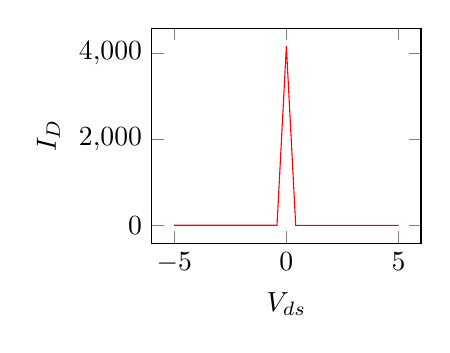
\begin{tikzpicture}
  \begin{axis}[
   xlabel=\begin{math}V_{ds}\end{math},
   ylabel=\begin{math}I_D\end{math},
   ]
   \addplot[
   color=red]
   {-1/(3*x)};
  \end{axis}

 \end{tikzpicture} &
 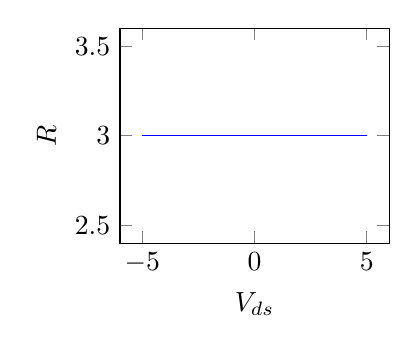
\begin{tikzpicture}
  \begin{axis}[
   xlabel=\begin{math}V_{ds}\end{math},
   ylabel=\begin{math}R\end{math},
   ]
   \addplot[
   color=blue]
   {3};
  \end{axis}
 \end{tikzpicture} \\
 \hline
 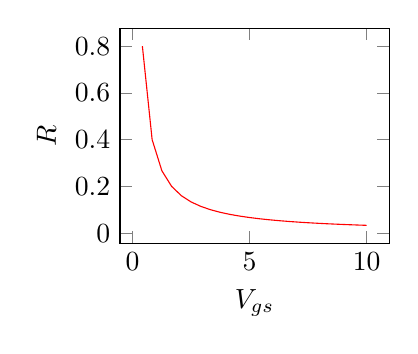
\begin{tikzpicture}
  \begin{axis}[
   domain=0:10,
   xlabel=\begin{math}V_{gs}\end{math},
   ylabel=\begin{math}R\end{math},
   ]
   \addplot[
   color=red]
   {1/(3*x)};
  \end{axis}

 \end{tikzpicture} &
 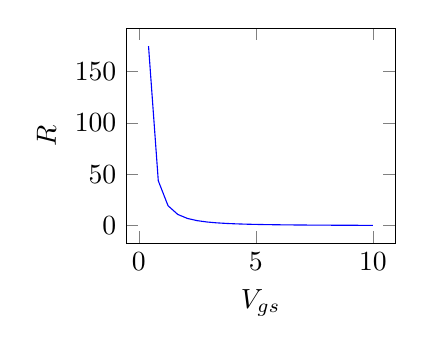
\begin{tikzpicture}
  \begin{axis}[
   domain=0:10,
   xlabel=\begin{math}V_{gs}\end{math},
   ylabel=\begin{math}R\end{math},
   ]
   \addplot[
   color=blue]
   {1/(0.033*x^2)};
  \end{axis}
 \end{tikzpicture} \\
 \hline
\end{tabular}
\section*{Problem - 3}
While \begin{math}V_{gs} < V_T\end{math},
\begin{equation}
 I_{DS} = I_0 exp\left(\frac{q(V_{gs} - V_T)}{nk_B T}\right)\left(1 - exp\left(- \frac{qV_{ds}}{k_B T}\right)\right)
\end{equation}
As \begin{math}V_{ds} >> k_B T/q\end{math}
\begin{equation}
 I_{DS} = I_0 exp\left(\frac{q(V_{gs} - V_T)}{nk_B T}\right)(1 - exp(-V_{ds}))
\end{equation}
\begin{tabular}{|c|}
\hline
 \begin{math}V_{gs} < V_T \end{math} (OFF conditions) and assume \begin{math}V_{ds} >> k_B T/q\end{math}\\
 \hline
 \begin{math}\frac{\partial I_{DS}}{\partial V_g} = I_0 (1 - exp(-V_{ds}))\frac{q}{nk_B T} exp\left(\frac{q(V_{gs} - V_T)}{nk_B T}\right)\end{math}\\
 \hline
 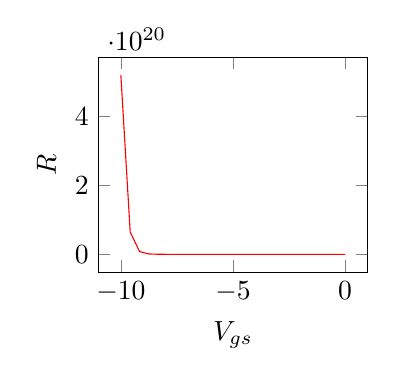
\begin{tikzpicture}
  \begin{axis}[
  domain=-10:0,
   xlabel=\begin{math}V_{gs}\end{math},
   ylabel=\begin{math}R\end{math},
   ]
   \addplot[
   color=red]
   {1/(10*exp(5*x))};
  \end{axis}
 \end{tikzpicture}\\
 \hline
\end{tabular}
\\
\\
\\
\begin{tabular}{|c|c|}
 \hline
 \multicolumn{2}{|c|}{\begin{math}V_{gs} > V_T\end{math} (ON conditions)} \\
 \hline
 Linear operation & Saturation operation \\
 \hline
 \begin{math}\frac{\partial I_{DS}}{\partial V_g} = \mu C_{ox} V_{ds} \left( \frac{W}{L} \right)\end{math} &
 \begin{math}\frac{\partial I_{DS}}{\partial V_g} = \mu C_{ox} \left( \frac{W}{L} \right) (V_{gs} - V_T) (1 + \lambda V_{ds})\end{math}\\
 \hline
  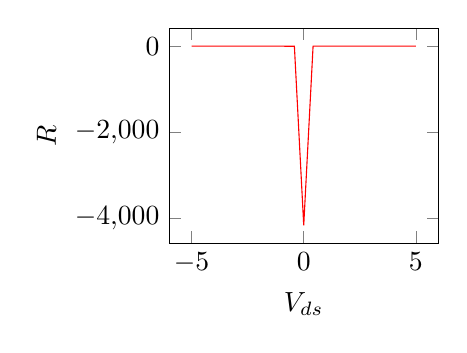
\begin{tikzpicture}
  \begin{axis}[
   xlabel=\begin{math}V_{ds}\end{math},
   ylabel=\begin{math}R\end{math},
   ]
   \addplot[
   color=red]
   {1/(3*x)};
  \end{axis}

 \end{tikzpicture} &
 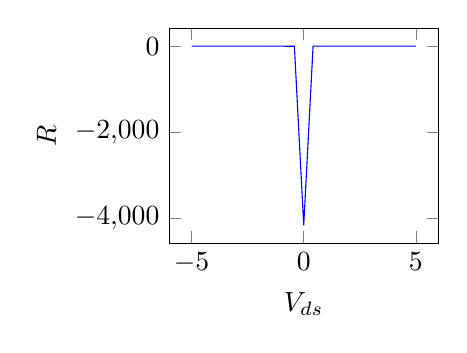
\begin{tikzpicture}
  \begin{axis}[
   xlabel=\begin{math}V_{ds}\end{math},
   ylabel=\begin{math}R\end{math},
   ]
   \addplot[
   color=blue]
   {1/(3*x)};
  \end{axis}
 \end{tikzpicture} \\
 \hline
 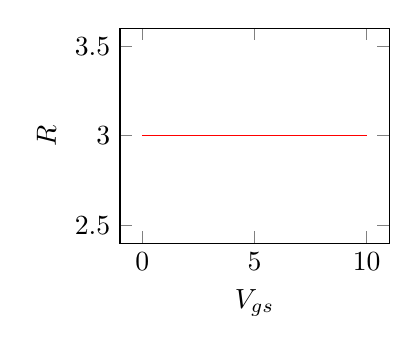
\begin{tikzpicture}
  \begin{axis}[
   domain=0:10,
   xlabel=\begin{math}V_{gs}\end{math},
   ylabel=\begin{math}R\end{math},
   ]
   \addplot[
   color=red]
   {3};
  \end{axis}

 \end{tikzpicture} &
 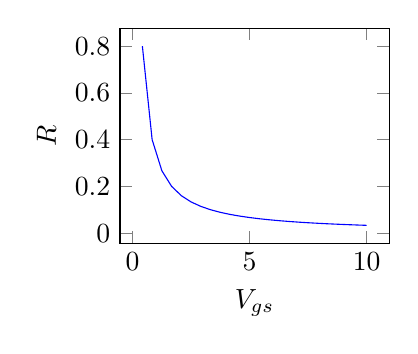
\begin{tikzpicture}
  \begin{axis}[
   domain=0:10,
   xlabel=\begin{math}V_{gs}\end{math},
   ylabel=\begin{math}R\end{math},
   ]
   \addplot[
   color=blue]
   {1/(3*x)};
  \end{axis}
 \end{tikzpicture} \\
 \hline
\end{tabular}
\end{document}
